\documentclass{amsart}


%%%%%%% Standard Packages
\usepackage{amsmath}       % I think this gives me some symbols
\usepackage{amsthm}        % Does theorem stuff
\usepackage{amssymb}       % more symbols and fonts
\usepackage{amsfonts}
\usepackage[all]{xy}
\usepackage{xspace}
\usepackage{calc}



\setlength{\topskip}{0pt}
\setlength{\footskip}{30pt}
\headheight=0pt
\topmargin=0pt
\headsep=18pt
\textheight=603pt %% 792pt to page, 648 is 9in
\textwidth=420pt  %% 612pt to page, 468pt is 6.5in
\oddsidemargin=25pt
\evensidemargin=25pt

\pagestyle{plain}


%%%%%% Adds hyperlinks
\usepackage[colorlinks, linkcolor=black, citecolor=blue,
	% pagebackref,
 	%bookmarksnumbered=true
	]{hyperref}
	
	
	
%%%%%% Tikz !!! Commands and Macros %%%%%%%%%%%%%
\usepackage{tikz}
\usetikzlibrary{matrix}


%%%% These draw triple or quadruple set of arrows of length 0.5 cm
\DeclareMathOperator{\righttriplearrows} {{\; \tikz{ \foreach \y in {0, 0.1, 0.2} { \draw [-stealth] (0, \y) -- +(0.5, 0);}} \; }}
\DeclareMathOperator{\lefttriplearrows} {{\; \tikz{ \foreach \y in {0, 0.1, 0.2} { \draw [stealth-] (0, \y) -- +(0.5, 0);}} \; }}
\DeclareMathOperator{\rightquadarrows} {{\; \tikz{ \foreach \y in {0, 0.1, 0.2, 0.3} { \draw [-stealth] (0, \y) -- +(0.5, 0);}} \; }}
\DeclareMathOperator{\leftquadarrows} {{\; \tikz{ \foreach \y in {0, 0.1, 0.2, 0.3} { \draw [stealth-] (0, \y) -- +(0.5, 0);}} \; }}

%%%%%%% End TikZ Commands and Macros %%%%%%%%%%%%%



%%%%%%%%%%%%%%%%%%%%%% Theorem Styles and Counters %%%%%%%%%%%%%%%%%%%%%%%%%%
% These all use the same "theorem" counter. 
\theoremstyle{plain} %%% Plain Theorem Styles.
\newtheorem{theorem}{Theorem}[section]
\newtheorem{lemma}[theorem]{Lemma}
\newtheorem{corollary}[theorem]{Corollary}          
\newtheorem{proposition}[theorem]{Proposition}              

\theoremstyle{definition} %%%% Definition-like Commands  
\newtheorem{definition}[theorem]{Definition}

\theoremstyle{remark}  %%%% Remark-like Commands
\newtheorem{remark}[theorem]{Remark}
\newtheorem{example}[theorem]{Example}
%%%%%%%%%%%%%%%%%%%%%% End Theorem Styles and Counters %%%%%%%%%%%%%%%%%%%%%%%%%%

%%%% Misc symbols %%%%%

\newcommand{\nn}{\nonumber}
\newcommand{\nid}{\noindent}
\newcommand{\ra}{\rightarrow}
\newcommand{\la}{\leftarrow}
\newcommand{\xra}{\xrightarrow}
\newcommand{\xla}{\xleftarrow}

\newcommand{\Bord}{\mathrm{Bord}}
\newcommand{\Vect}{\mathrm{Vect}}
\newcommand{\TC}{\mathrm{TC}}

\def\cA{\mathcal A}\def\cB{\mathcal B}\def\cC{\mathcal C}\def\cD{\mathcal D}
\def\cE{\mathcal E}\def\cF{\mathcal F}\def\cG{\mathcal G}\def\cH{\mathcal H}
\def\cI{\mathcal I}\def\cJ{\mathcal J}\def\cK{\mathcal K}\def\cL{\mathcal L}
\def\cM{\mathcal M}\def\cN{\mathcal N}\def\cO{\mathcal O}\def\cP{\mathcal P}
\def\cQ{\mathcal Q}\def\cR{\mathcal R}\def\cS{\ess}\def\cT{\mathcal T}
\def\cU{\mathcal U}\def\cV{\mathcal V}\def\cW{\mathcal W}\def\cX{\mathcal X}
\def\cY{\mathcal Y}\def\cZ{\mathcal Z}

\def\AA{\mathbb A}\def\BB{\mathbb B}\def\CC{\mathbb C}\def\DD{\mathbb D}
\def\EE{\mathbb E}\def\FF{\mathbb F}\def\GG{\mathbb G}\def\HH{\mathbb H}
\def\II{\mathbb I}\def\JJ{\mathbb J}\def\KK{\mathbb K}\def\LL{\mathbb L}
\def\MM{\mathbb M}\def\NN{\mathbb N}\def\OO{\mathbb O}\def\PP{\mathbb P}
\def\QQ{\mathbb Q}\def\RR{\mathbb R}\def\SS{\mathbb S}\def\TT{\mathbb T}
\def\UU{\mathbb U}\def\VV{\mathbb V}\def\WW{\mathbb W}\def\XX{\mathbb X}
\def\YY{\mathbb Y}\def\ZZ{\mathbb Z}

%%%%%%%%%
















\usepgflibrary{decorations.pathreplacing}

\begin{document}
	
	\title{Sandbox}
	
	\maketitle

\section{Bordism pics}

%\begin{figure}[htbp]
%	\begin{center}
%		\begin{tikzpicture}[
%			% This decoration will be used to make portions of curves into "bouckground curves". It allows us to dash a portion of the curve.
%			decoration={border, 
%				segment length = 4pt, 	% determines the distance between consecutive ticks.
%				amplitude = 2pt, 		% determines the length of the ticks.
%				angle = 0  				% determines the angle between the ticks and the line of the path. 
%				}, 
%			% Styles
%			contour line/.style={thin, blue}
%				]
%				
%			% Colors
%			\colorlet{surfacecolor1}{blue!15}
%			\colorlet{surfacecolor2}{blue!10}	
%			
%			% The graphic
%			\draw [step = 1cm, help lines] (-0.9,-0.9) grid (11.9, 10.9);
%			
%			% First we fill the surfaces with the background colors.
%			% region 1
%			\fill [color = surfacecolor1] (0, 2.5) .. controls (0, 4) and (2,6.5) .. (1.75,8)
%				arc (180:0:2cm and 3cm)
%				%.. controls (3, 9) and (3,10) .. (4,10)
%				%.. controls (4.5,10) and (6,9.5) .. (6,8)
%				to [out = 270, in = 90] (6, 5.5)
%				-- (6,0.5)
%				arc (360: 180: 1cm and 0.5cm)
%				-- (4, 6)
%				arc (90:180:2cm and 3.5cm)
%				%.. controls (1, 2) and (1.5, 2) .. (1, 2)
%				to [out = 210, in = 0] (1,2)
%				arc (270: 180: 1cm and 0.5cm);
%			
%			% region 2
%			\fill [color = surfacecolor1] (7, 6.5) parabola bend (8.5, 5.8) (8.25, 5.8) 
%				to [out = 45, in = 260] (9, 7)
%				parabola bend (7.75, 6.4) (7, 6.5);
%			
%			% region 3
%			\fill [color = surfacecolor2] (4, 6) arc (90:180:2cm and 3.5cm)
%				-- (4, 1.5) -- (4,6);
%			
%			% region 4
%			\fill [color = surfacecolor2] (6, 5.5) parabola (7, 6.5) parabola bend (8.5, 5.8) (11, 6)
%				to [out = 240, in = 30] (8, 2.5) -- (6, 1.5) -- (6, 5.5);
%			
%			
%			% Now we draw the lines of the surface
%			%first around region 1
%			\draw (0, 2.5) .. controls (0, 4) and (2,6.5) .. (1.75,8)
%				arc (180:0:2cm and 3cm)
%				%.. controls (3, 9) and (3,10) .. (4,10)
%				%.. controls (4.5,10) and (6,9.5) .. (6,8)
%				to [out = 270, in = 90] (6, 5.5)
%				-- (6,0.5)
%				arc (360: 180: 1cm and 0.5cm)
%				-- (4, 6)
%				arc (90:180:2cm and 3.5cm)
%				%.. controls (1, 2) and (1.5, 2) .. (1, 2)
%				to [out = 210, in = 0] (1,2)
%				arc (270: 180: 1cm and 0.5cm);
%			
%			% then the rest 
%			\draw (2,2.5) -- (4,1.5) 
%				decorate {-- (5,1) to [out = -30, in = 135] (6,0.5)
%					  (4,0.5) to [out = 45, in = 210] (5,1) -- (6,1.5)} 
%				-- (8, 2.5) to [out = 30, in = 240] (11, 6);
%				% then off to cusp points
%			\draw decorate { (5, 1) arc (0:90:1cm and 5cm)};
%			\draw decorate {(2,2.5) -- (7,5) to [out = 30, in = 225] (8.25, 5.8)} to [out = 45, in = 260] (9, 7) ;
%			\draw decorate {(2,2.5) to [out = 150, in = 0] (1,3) arc (90:180:1cm and 0.5cm)};
%			% cusp
%			\draw (4, 6) to [out = 90, in = 270] (4.5, 8.5);
%			\draw (6, 5.5) decorate { parabola (4.5, 8.5)} (6, 5.5) parabola (7, 6.5)
%				parabola bend (7.75, 6.4) (9, 7);
%			\draw (7, 6.5) parabola bend (8.5, 5.8) (11, 6);
%			
%%		% now the contour lines
%%		% the first contour line
%%		\draw [contour line] (2.25, 10) arc (180:360:1.5cm and 0.5cm)
%%			decorate {(2.25, 10) arc (180:0:1.5cm and 0.5cm)};
%%		
%%		
%%		% the second contour line
%%		
%%		% the third contour line
%%		\draw [contour line] 
%%			decorate {(1.25, 5.75) arc (180:90: 1cm and 0.5cm) to [out = 0, in = 150] (3.5,5.75)}
%%			 -- (4, 5.5) 
%%			decorate {-- (4.5,5.25) to [out = -30, in = 135] (6,5)}
%%			arc (360: 180: 1cm and 0.5cm)
%%			decorate { to [out = 45, in = 210] (4.5,5.25)};
%%		
%%		\draw [contour line] 
%%		 (1.25, 5.75) arc (180: 270: 1cm and 0.5cm) to [out = 0, in = 210] (3.25,5.75)
%%		 	 to [out = 30, in = 150] (5.25, 6.15) to [out = -30,in = 30] (4.5, 5.25);
%			
%			%\draw (0,3) decorate {to (2,3)} -- (3,4);
%				
%		\end{tikzpicture}
%		\end{center}	
%	\caption{Without contour lines}
%	%\label{fig:label}
%\end{figure}

%\begin{figure}[htbp]
%	\begin{center}
%		\begin{tikzpicture}[
%			% This decoration will be used to make portions of curves into "bouckground curves". It allows us to dash a portion of the curve.
%			decoration={border, 
%				segment length = 4pt, 	% determines the distance between consecutive ticks.
%				amplitude = 2pt, 		% determines the length of the ticks.
%				angle = 0  				% determines the angle between the ticks and the line of the path. 
%				}, 
%			% Styles
%			contour line/.style={thin, blue}
%				]
%				
%			% Colors
%			\colorlet{surfacecolor1}{blue!15}
%			\colorlet{surfacecolor2}{blue!10}	
%			
%			% The graphic
%			\draw [step = 1cm, help lines] (-0.9,-0.9) grid (11.9, 10.9);
%			
%			% First we fill the surfaces with the background colors.
%			% region 1
%			\fill [color = surfacecolor1] (0, 2.5) .. controls (0, 4) and (2,6.5) .. (1.75,8)
%				arc (180:0:2cm and 3cm)
%				%.. controls (3, 9) and (3,10) .. (4,10)
%				%.. controls (4.5,10) and (6,9.5) .. (6,8)
%				to [out = 270, in = 90] (6, 5.5)
%				-- (6,0.5)
%				arc (360: 180: 1cm and 0.5cm)
%				-- (4, 6)
%				arc (90:180:2cm and 3.5cm)
%				%.. controls (1, 2) and (1.5, 2) .. (1, 2)
%				to [out = 210, in = 0] (1,2)
%				arc (270: 180: 1cm and 0.5cm);
%			
%			% region 2
%			\fill [color = surfacecolor1] (7, 6.5) parabola bend (8.5, 5.8) (8.25, 5.8) 
%				to [out = 45, in = 260] (9, 7)
%				parabola bend (7.75, 6.4) (7, 6.5);
%			
%			% region 3
%			\fill [color = surfacecolor2] (4, 6) arc (90:180:2cm and 3.5cm)
%				-- (4, 1.5) -- (4,6);
%			
%			% region 4
%			\fill [color = surfacecolor2] (6, 5.5) parabola (7, 6.5) parabola bend (8.5, 5.8) (11, 6)
%				to [out = 240, in = 30] (8, 2.5) -- (6, 1.5) -- (6, 5.5);
%			
%			
%			% Now we draw the lines of the surface
%			%first around region 1
%			\draw (0, 2.5) .. controls (0, 4) and (2,6.5) .. (1.75,8)
%				arc (180:0:2cm and 3cm)
%				%.. controls (3, 9) and (3,10) .. (4,10)
%				%.. controls (4.5,10) and (6,9.5) .. (6,8)
%				to [out = 270, in = 90] (6, 5.5)
%				-- (6,0.5)
%				arc (360: 180: 1cm and 0.5cm)
%				-- (4, 6)
%				arc (90:180:2cm and 3.5cm)
%				%.. controls (1, 2) and (1.5, 2) .. (1, 2)
%				to [out = 210, in = 0] (1,2)
%				arc (270: 180: 1cm and 0.5cm);
%			
%			% then the rest 
%			\draw (2,2.5) -- (4,1.5) 
%				decorate {-- (5,1) to [out = -30, in = 135] (6,0.5)
%					  (4,0.5) to [out = 45, in = 210] (5,1) -- (6,1.5)} 
%				-- (8, 2.5) to [out = 30, in = 240] (11, 6);
%				% then off to cusp points
%			\draw decorate { (5, 1) arc (0:90:1cm and 5cm)};
%			\draw decorate {(2,2.5) -- (7,5) to [out = 30, in = 225] (8.25, 5.8)} to [out = 45, in = 260] (9, 7) ;
%			\draw decorate {(2,2.5) to [out = 150, in = 0] (1,3) arc (90:180:1cm and 0.5cm)};
%			% cusp
%			\draw (4, 6) to [out = 90, in = 270] (4.5, 8.5);
%			\draw (6, 5.5) decorate { parabola (4.5, 8.5)} (6, 5.5) parabola (7, 6.5)
%				parabola bend (7.75, 6.4) (9, 7);
%			\draw (7, 6.5) parabola bend (8.5, 5.8) (11, 6);
%			
%			% now the contour lines
%			% the first contour line
%			\draw [contour line] (2.3, 10) arc (180:360:1.45cm and 0.5cm)
%				decorate {(2.3, 10) arc (180:0:1.45cm and 0.5cm)};
%			
%			
%			% the second contour line
%			\draw [contour line] (1.75,8) arc (180:320:1.45cm and 0.5cm)
%				decorate {to [out = 30,in = 135](4.65, 7.6) to [out = -45, in = 45] (4.2, 7.1) }
%				arc (180:270:0.5cm and 0.2cm) to [out = 0, in = -90] (5.75,8)
%			;
%			\draw [contour line] decorate {(1.75,8) arc (180:0:2cm and 0.6cm)};
%			
%			% the third contour line
%			\draw [contour line] 
%				decorate {(1.25, 5.75) arc (180:90: 1cm and 0.5cm) to [out = 0, in = 150] (3.5,5.75)}
%				 -- (4, 5.5) 
%				decorate {-- (4.5,5.25) to [out = -30, in = 135] (6,5)}
%				arc (360: 180: 1cm and 0.5cm)
%				decorate { to [out = 45, in = 210] (4.5,5.25)};
%			
%			\draw [contour line] 
%			 (1.25, 5.75) arc (180: 270: 1cm and 0.5cm) to [out = 0, in = 210] (3.25,5.75)
%			 	 to [out = 30, in = 150] (5.25, 6.15) to [out = -30,in = 30] (4.5, 5.25);
%			
%			%\draw (0,3) decorate {to (2,3)} -- (3,4);
%				
%		\end{tikzpicture}
%		\end{center}	
%	\caption{with contour lines}
%	%\label{fig:label}
%\end{figure}

\begin{figure}[htbp]
	\begin{center}
		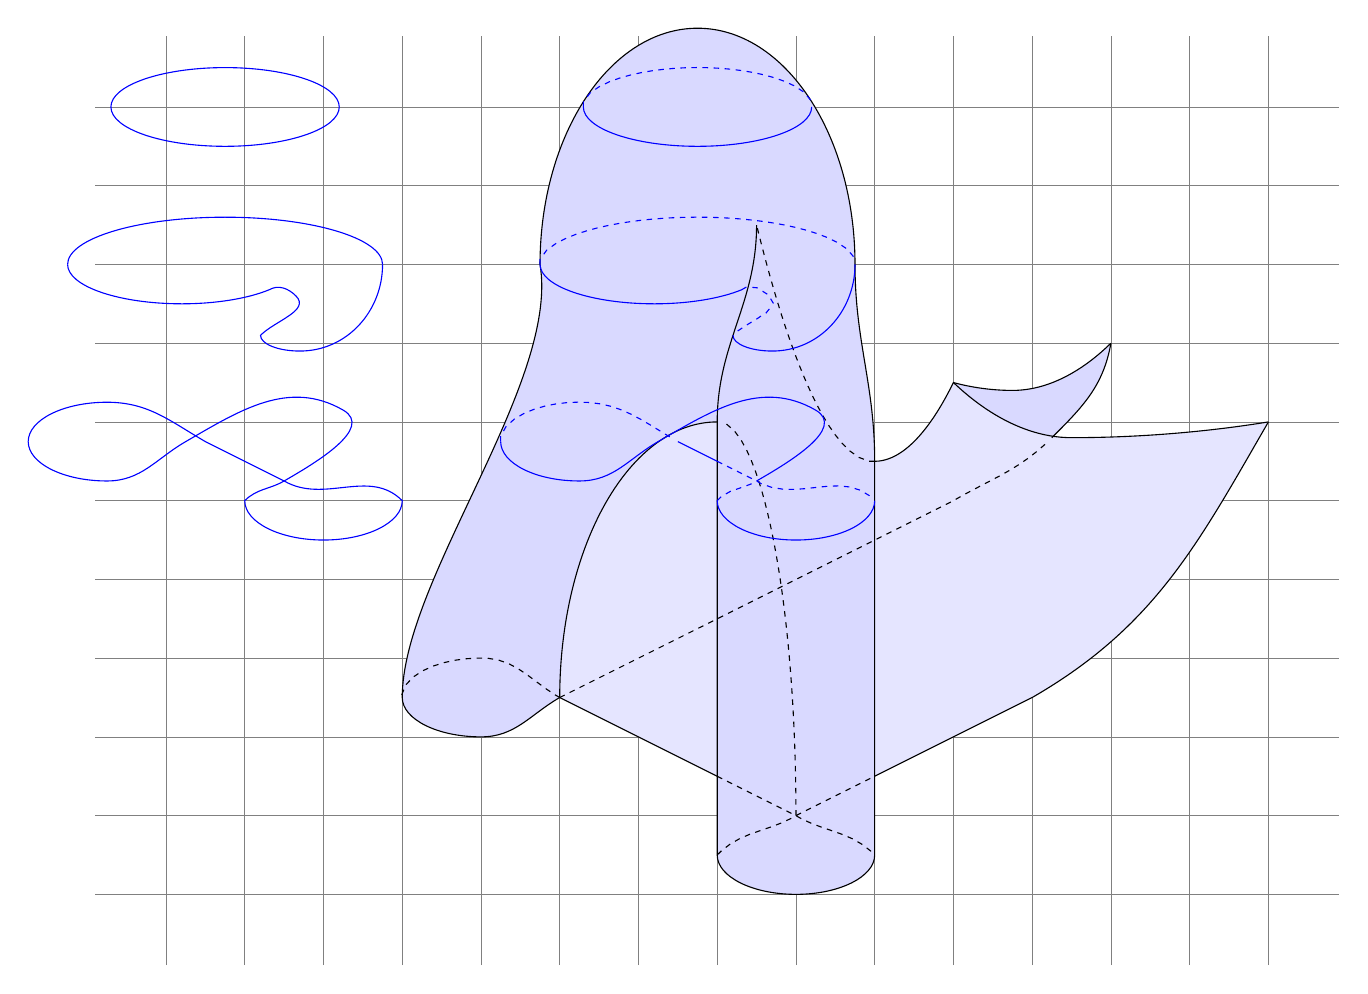
\begin{tikzpicture}[
			% This decoration will be used to make portions of curves into "bouckground curves". It allows us to dash a portion of the curve.
			decoration={border, 
				segment length = 4pt, 	% determines the distance between consecutive ticks.
				amplitude = 2pt, 		% determines the length of the ticks.
				angle = 0  				% determines the angle between the ticks and the line of the path. 
				}, 
			% Styles
			contour line/.style={thin, blue}
				]
				
			% Colors
			\colorlet{surfacecolor1}{blue!15}
			\colorlet{surfacecolor2}{blue!10}	
			
			% The graphic
			\draw [step = 1cm, help lines] (-3.9,-0.9) grid (11.9, 10.9);
			
			% First we fill the surfaces with the background colors.
			% region 1
			\fill [color = surfacecolor1] (0, 2.5) .. controls (0, 4) and (2,6.5) .. (1.75,8)
				arc (180:0:2cm and 3cm)
				%.. controls (3, 9) and (3,10) .. (4,10)
				%.. controls (4.5,10) and (6,9.5) .. (6,8)
				to [out = 270, in = 90] (6, 5.5)
				-- (6,0.5)
				arc (360: 180: 1cm and 0.5cm)
				-- (4, 6)
				arc (90:180:2cm and 3.5cm)
				%.. controls (1, 2) and (1.5, 2) .. (1, 2)
				to [out = 210, in = 0] (1,2)
				arc (270: 180: 1cm and 0.5cm);
			
			% region 2
			\fill [color = surfacecolor1] (7, 6.5) parabola bend (8.5, 5.8) (8.25, 5.8) 
				to [out = 45, in = 260] (9, 7)
				parabola bend (7.75, 6.4) (7, 6.5);
			
			% region 3
			\fill [color = surfacecolor2] (4, 6) arc (90:180:2cm and 3.5cm)
				-- (4, 1.5) -- (4,6);
			
			% region 4
			\fill [color = surfacecolor2] (6, 5.5) parabola (7, 6.5) parabola bend (8.5, 5.8) (11, 6)
				to [out = 240, in = 30] (8, 2.5) -- (6, 1.5) -- (6, 5.5);
			
			
			% Now we draw the lines of the surface
			%first around region 1
			\draw (0, 2.5) .. controls (0, 4) and (2,6.5) .. (1.75,8)
				arc (180:0:2cm and 3cm)
				%.. controls (3, 9) and (3,10) .. (4,10)
				%.. controls (4.5,10) and (6,9.5) .. (6,8)
				to [out = 270, in = 90] (6, 5.5)
				-- (6,0.5)
				arc (360: 180: 1cm and 0.5cm)
				-- (4, 6)
				arc (90:180:2cm and 3.5cm)
				%.. controls (1, 2) and (1.5, 2) .. (1, 2)
				to [out = 210, in = 0] (1,2)
				arc (270: 180: 1cm and 0.5cm);
			
			% then the rest 
			\draw (2,2.5) -- (4,1.5) 
				decorate {-- (5,1) to [out = -30, in = 135] (6,0.5)
					  (4,0.5) to [out = 45, in = 210] (5,1) -- (6,1.5)} 
				-- (8, 2.5) to [out = 30, in = 240] (11, 6);
				% then off to cusp points
			\draw decorate { (5, 1) arc (0:90:1cm and 5cm)};
			\draw decorate {(2,2.5) -- (7,5) to [out = 30, in = 225] (8.25, 5.8)} to [out = 45, in = 260] (9, 7) ;
			\draw decorate {(2,2.5) to [out = 150, in = 0] (1,3) arc (90:180:1cm and 0.5cm)};
			% cusp
			\draw (4, 6) to [out = 90, in = 270] (4.5, 8.5);
			\draw (6, 5.5) decorate { parabola (4.5, 8.5)} (6, 5.5) parabola (7, 6.5)
				parabola bend (7.75, 6.4) (9, 7);
			\draw (7, 6.5) parabola bend (8.5, 5.8) (11, 6);
			
			% now the contour lines
			% the first contour line
			\draw [contour line] (2.3, 10) arc (180:360:1.45cm and 0.5cm)
				decorate {(2.3, 10) arc (180:0:1.45cm and 0.5cm)};
			
			
			% the second contour line
			\draw [contour line] (1.75,8) arc (180:320:1.45cm and 0.5cm)
				decorate {to [out = 30,in = 135](4.65, 7.6) to [out = -45, in = 45] (4.2, 7.1) }
				arc (180:270:0.5cm and 0.2cm) to [out = 0, in = -90] (5.75,8)
			;
			\draw [contour line] decorate {(1.75,8) arc (180:0:2cm and 0.6cm)};
			
			% the third contour line
			\draw [contour line] 
				decorate {(1.25, 5.75) arc (180:90: 1cm and 0.5cm) to [out = 0, in = 150] (3.5,5.75)}
				 -- (4, 5.5) 
				decorate {-- (4.5,5.25) to [out = -30, in = 135] (6,5)}
				arc (360: 180: 1cm and 0.5cm)
				decorate { to [out = 45, in = 210] (4.5,5.25)};
			
			\draw [contour line] 
			 (1.25, 5.75) arc (180: 270: 1cm and 0.5cm) to [out = 0, in = 210] (3.25,5.75)
			 	 to [out = 30, in = 150] (5.25, 6.15) to [out = -30,in = 30] (4.5, 5.25);
			
			
			\begin{scope}[xshift = -6cm]
				% now the contour lines
				% the first contour line
				\draw [contour line] (2.3, 10) arc (180:360:1.45cm and 0.5cm)
					 {(2.3, 10) arc (180:0:1.45cm and 0.5cm)};
			
			
				% the second contour line
				\draw [contour line] (1.75,8) arc (180:320:1.45cm and 0.5cm)
					 {to [out = 30,in = 135](4.65, 7.6) to [out = -45, in = 45] (4.2, 7.1) }
					arc (180:270:0.5cm and 0.2cm) to [out = 0, in = -90] (5.75,8)
				;
				\draw [contour line]  {(1.75,8) arc (180:0:2cm and 0.6cm)};
			
				% the third contour line
				\draw [contour line] 
					 {(1.25, 5.75) arc (180:90: 1cm and 0.5cm) to [out = 0, in = 150] (3.5,5.75)}
					 -- (4, 5.5) 
					 {-- (4.5,5.25) to [out = -30, in = 135] (6,5)}
					arc (360: 180: 1cm and 0.5cm)
					 { to [out = 45, in = 210] (4.5,5.25)};
			
				\draw [contour line] 
				 (1.25, 5.75) arc (180: 270: 1cm and 0.5cm) to [out = 0, in = 210] (3.25,5.75)
				 	 to [out = 30, in = 150] (5.25, 6.15) to [out = -30,in = 30] (4.5, 5.25);
			\end{scope}
			
			
			
							
		\end{tikzpicture}
		\end{center}	
	\caption{with contour lines and translated contour lines}
	%\label{fig:label}
\end{figure}



\begin{figure}[htbp]
	\begin{center}
		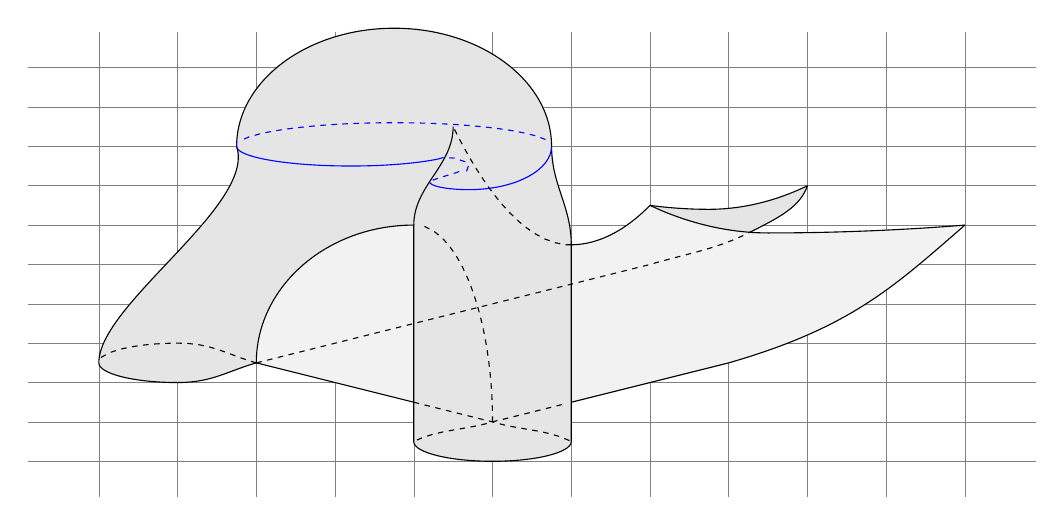
\begin{tikzpicture}[
			yscale=0.5,
			% This decoration will be used to make portions of curves into "bouckground curves". It allows us to dash a portion of the curve.
			decoration={border, 
				segment length = 4pt, 	% determines the distance between consecutive ticks.
				amplitude = 2pt, 		% determines the length of the ticks.
				angle = 0  				% determines the angle between the ticks and the line of the path. 
				}, 
			% Styles
			contour line/.style={thin, blue}
				]
				
			% Colors
			\colorlet{surfacecolor1}{black!10}
			\colorlet{surfacecolor2}{black!5}	
			
			% The graphic
			\draw [step = 1cm, help lines] (-0.9,-0.9) grid (11.9, 10.9);
			
			% First we fill the surfaces with the background colors.
			% region 1
			\fill [color = surfacecolor1] (0, 2.5) .. controls (0, 4) and (2,6.5) .. (1.75,8)
				arc (180:0:2cm and 3cm)
				%.. controls (3, 9) and (3,10) .. (4,10)
				%.. controls (4.5,10) and (6,9.5) .. (6,8)
				to [out = 270, in = 90] (6, 5.5)
				-- (6,0.5)
				arc (360: 180: 1cm and 0.5cm)
				-- (4, 6)
				arc (90:180:2cm and 3.5cm)
				%.. controls (1, 2) and (1.5, 2) .. (1, 2)
				to [out = 210, in = 0] (1,2)
				arc (270: 180: 1cm and 0.5cm);
			
			% region 2
			\fill [color = surfacecolor1] (7, 6.5) parabola bend (8.5, 5.8) (8.25, 5.8) 
				to [out = 45, in = 260] (9, 7)
				parabola bend (7.75, 6.4) (7, 6.5);
			
			% region 3
			\fill [color = surfacecolor2] (4, 6) arc (90:180:2cm and 3.5cm)
				-- (4, 1.5) -- (4,6);
			
			% region 4
			\fill [color = surfacecolor2] (6, 5.5) parabola (7, 6.5) parabola bend (8.5, 5.8) (11, 6)
				to [out = 240, in = 30] (8, 2.5) -- (6, 1.5) -- (6, 5.5);
			
			
			% Now we draw the lines of the surface
			%first around region 1
			\draw (0, 2.5) .. controls (0, 4) and (2,6.5) .. (1.75,8)
				arc (180:0:2cm and 3cm)
				%.. controls (3, 9) and (3,10) .. (4,10)
				%.. controls (4.5,10) and (6,9.5) .. (6,8)
				to [out = 270, in = 90] (6, 5.5)
				-- (6,0.5)
				arc (360: 180: 1cm and 0.5cm)
				-- (4, 6)
				arc (90:180:2cm and 3.5cm)
				%.. controls (1, 2) and (1.5, 2) .. (1, 2)
				to [out = 210, in = 0] (1,2)
				arc (270: 180: 1cm and 0.5cm);
			
			% then the rest 
			\draw (2,2.5) -- (4,1.5) 
				decorate {-- (5,1) to [out = -30, in = 135] (6,0.5)
					  (4,0.5) to [out = 45, in = 210] (5,1) -- (6,1.5)} 
				-- (8, 2.5) to [out = 30, in = 240] (11, 6);
				% then off to cusp points
			\draw decorate { (5, 1) arc (0:90:1cm and 5cm)};
			\draw decorate {(2,2.5) -- (7,5) to [out = 30, in = 225] (8.25, 5.8)} to [out = 45, in = 260] (9, 7) ;
			\draw decorate {(2,2.5) to [out = 150, in = 0] (1,3) arc (90:180:1cm and 0.5cm)};
			% cusp
			\draw (4, 6) to [out = 90, in = 270] (4.5, 8.5);
			\draw (6, 5.5) decorate { parabola (4.5, 8.5)} (6, 5.5) parabola (7, 6.5)
				parabola bend (7.75, 6.4) (9, 7);
			\draw (7, 6.5) parabola bend (8.5, 5.8) (11, 6);
			
%		% now the contour lines
%		% the first contour line
%		\draw [contour line] (2.25, 10) arc (180:360:1.5cm and 0.5cm)
%			decorate {(2.25, 10) arc (180:0:1.5cm and 0.5cm)};
%		
%		
%		% the second contour line
		\draw [contour line] (1.75,8) arc (180:320:1.45cm and 0.5cm)
			decorate {to [out = 30,in = 135](4.65, 7.6) to [out = -45, in = 45] (4.2, 7.1) }
			arc (180:270:0.5cm and 0.2cm) to [out = 0, in = -90] (5.75,8)
		;
		\draw [contour line] decorate {(1.75,8) arc (180:0:2cm and 0.6cm)};
%		% the third contour line
%		\draw [contour line] 
%			decorate {(1.25, 5.75) arc (180:90: 1cm and 0.5cm) to [out = 0, in = 150] (3.5,5.75)}
%			 -- (4, 5.5) 
%			decorate {-- (4.5,5.25) to [out = -30, in = 135] (6,5)}
%			arc (360: 180: 1cm and 0.5cm)
%			decorate { to [out = 45, in = 210] (4.5,5.25)};
%		
%		\draw [contour line] 
%		 (1.25, 5.75) arc (180: 270: 1cm and 0.5cm) to [out = 0, in = 210] (3.25,5.75)
%		 	 to [out = 30, in = 150] (5.25, 6.15) to [out = -30,in = 30] (4.5, 5.25);
			
			%\draw (0,3) decorate {to (2,3)} -- (3,4);
				
		\end{tikzpicture}
		\end{center}	
	\caption{Squashed version, with only one contour line. 
	 Maybe for the intro?}
	%\label{fig:label}
\end{figure}


\begin{figure}[htbp]
	\begin{center}
		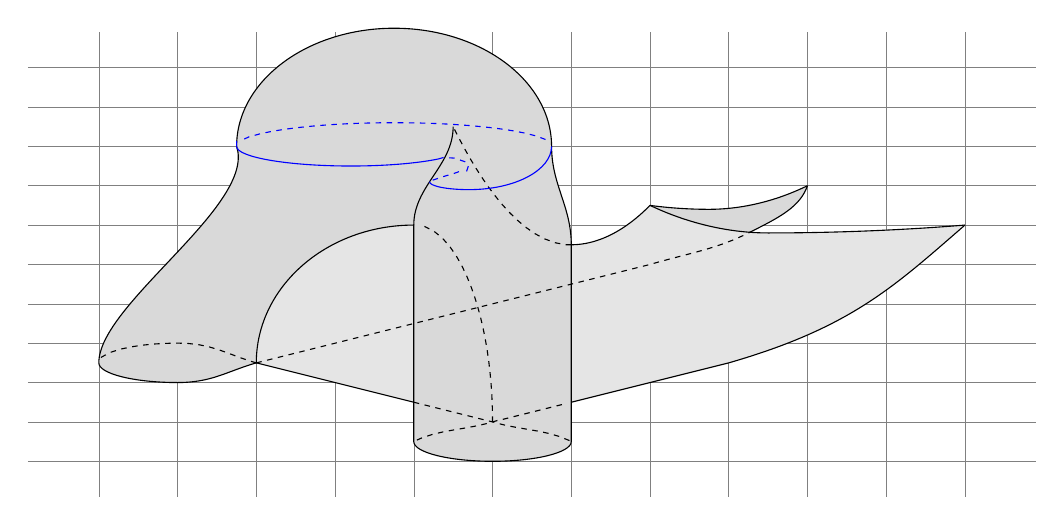
\begin{tikzpicture}[
			yscale=0.5,
			% This decoration will be used to make portions of curves into "bouckground curves". It allows us to dash a portion of the curve.
			decoration={border, 
				segment length = 4pt, 	% determines the distance between consecutive ticks.
				amplitude = 2pt, 		% determines the length of the ticks.
				angle = 0  				% determines the angle between the ticks and the line of the path. 
				}, 
			% Styles
			contour line/.style={thin, blue}
				]
				
			% Colors
			\colorlet{surfacecolor1}{black!15}
			\colorlet{surfacecolor2}{black!10}	
			
			% The graphic
			\draw [step = 1cm, help lines] (-0.9,-0.9) grid (11.9, 10.9);
			
			% First we fill the surfaces with the background colors.
			% region 1
			\fill [color = surfacecolor1] (0, 2.5) .. controls (0, 4) and (2,6.5) .. (1.75,8)
				arc (180:0:2cm and 3cm)
				%.. controls (3, 9) and (3,10) .. (4,10)
				%.. controls (4.5,10) and (6,9.5) .. (6,8)
				to [out = 270, in = 90] (6, 5.5)
				-- (6,0.5)
				arc (360: 180: 1cm and 0.5cm)
				-- (4, 6)
				arc (90:180:2cm and 3.5cm)
				%.. controls (1, 2) and (1.5, 2) .. (1, 2)
				to [out = 210, in = 0] (1,2)
				arc (270: 180: 1cm and 0.5cm);
			
			% region 2
			\fill [color = surfacecolor1] (7, 6.5) parabola bend (8.5, 5.8) (8.25, 5.8) 
				to [out = 45, in = 260] (9, 7)
				parabola bend (7.75, 6.4) (7, 6.5);
			
			% region 3
			\fill [color = surfacecolor2] (4, 6) arc (90:180:2cm and 3.5cm)
				-- (4, 1.5) -- (4,6);
			
			% region 4
			\fill [color = surfacecolor2] (6, 5.5) parabola (7, 6.5) parabola bend (8.5, 5.8) (11, 6)
				to [out = 240, in = 30] (8, 2.5) -- (6, 1.5) -- (6, 5.5);
			
			
			% Now we draw the lines of the surface
			%first around region 1
			\draw (0, 2.5) .. controls (0, 4) and (2,6.5) .. (1.75,8)
				arc (180:0:2cm and 3cm)
				%.. controls (3, 9) and (3,10) .. (4,10)
				%.. controls (4.5,10) and (6,9.5) .. (6,8)
				to [out = 270, in = 90] (6, 5.5)
				-- (6,0.5)
				arc (360: 180: 1cm and 0.5cm)
				-- (4, 6)
				arc (90:180:2cm and 3.5cm)
				%.. controls (1, 2) and (1.5, 2) .. (1, 2)
				to [out = 210, in = 0] (1,2)
				arc (270: 180: 1cm and 0.5cm);
			
			% then the rest 
			\draw (2,2.5) -- (4,1.5) 
				decorate {-- (5,1) to [out = -30, in = 135] (6,0.5)
					  (4,0.5) to [out = 45, in = 210] (5,1) -- (6,1.5)} 
				-- (8, 2.5) to [out = 30, in = 240] (11, 6);
				% then off to cusp points
			\draw decorate { (5, 1) arc (0:90:1cm and 5cm)};
			\draw decorate {(2,2.5) -- (7,5) to [out = 30, in = 225] (8.25, 5.8)} to [out = 45, in = 260] (9, 7) ;
			\draw decorate {(2,2.5) to [out = 150, in = 0] (1,3) arc (90:180:1cm and 0.5cm)};
			% cusp
			\draw (4, 6) to [out = 90, in = 270] (4.5, 8.5);
			\draw (6, 5.5) decorate { parabola (4.5, 8.5)} (6, 5.5) parabola (7, 6.5)
				parabola bend (7.75, 6.4) (9, 7);
			\draw (7, 6.5) parabola bend (8.5, 5.8) (11, 6);
			
%		% now the contour lines
%		% the first contour line
%		\draw [contour line] (2.25, 10) arc (180:360:1.5cm and 0.5cm)
%			decorate {(2.25, 10) arc (180:0:1.5cm and 0.5cm)};
%		
%		
%		% the second contour line
		\draw [contour line] (1.75,8) arc (180:320:1.45cm and 0.5cm)
			decorate {to [out = 30,in = 135](4.65, 7.6) to [out = -45, in = 45] (4.2, 7.1) }
			arc (180:270:0.5cm and 0.2cm) to [out = 0, in = -90] (5.75,8)
		;
		\draw [contour line] decorate {(1.75,8) arc (180:0:2cm and 0.6cm)};
%		% the third contour line
%		\draw [contour line] 
%			decorate {(1.25, 5.75) arc (180:90: 1cm and 0.5cm) to [out = 0, in = 150] (3.5,5.75)}
%			 -- (4, 5.5) 
%			decorate {-- (4.5,5.25) to [out = -30, in = 135] (6,5)}
%			arc (360: 180: 1cm and 0.5cm)
%			decorate { to [out = 45, in = 210] (4.5,5.25)};
%		
%		\draw [contour line] 
%		 (1.25, 5.75) arc (180: 270: 1cm and 0.5cm) to [out = 0, in = 210] (3.25,5.75)
%		 	 to [out = 30, in = 150] (5.25, 6.15) to [out = -30,in = 30] (4.5, 5.25);
			
			%\draw (0,3) decorate {to (2,3)} -- (3,4);
				
		\end{tikzpicture}
		\end{center}	
	\caption{Squashed version, with only one contour line, grayscale.}
	%\label{fig:label}
\end{figure}

%
%\begin{figure}[htbp]
%	\begin{center}
%		\begin{tikzpicture}[
%			% This decoration will be used to make portions of curves into "bouckground curves". It allows us to dash a portion of the curve.
%			decoration={border, 
%				segment length = 4pt, 	% determines the distance between consecutive ticks.
%				amplitude = 2pt, 		% determines the length of the ticks.
%				angle = 0  				% determines the angle between the ticks and the line of the path. 
%				}, 
%			% Styles
%			contour line/.style={thin, blue}
%				]
%				
%			% Colors
%			\colorlet{surfacecolor1}{blue!15}
%			\colorlet{surfacecolor2}{blue!10}	
%			
%			% The graphic
%			\draw [step = 1cm, help lines] (-3.9,-0.9) grid (11.9, 10.9);
%			
%			% First we fill the surfaces with the background colors.
%			% region 1
%			\fill [color = surfacecolor1] (0, 2.5) .. controls (0, 4) and (2,6.5) .. (1.75,8)
%				arc (180:0:2cm and 3cm)
%				%.. controls (3, 9) and (3,10) .. (4,10)
%				%.. controls (4.5,10) and (6,9.5) .. (6,8)
%				to [out = 270, in = 90] (6, 5.5)
%				-- (6,0.5)
%				arc (360: 180: 1cm and 0.5cm)
%				-- (4, 6)
%				arc (90:180:2cm and 3.5cm)
%				%.. controls (1, 2) and (1.5, 2) .. (1, 2)
%				to [out = 210, in = 0] (1,2)
%				arc (270: 180: 1cm and 0.5cm);
%			
%			% region 2
%			\fill [color = surfacecolor1] (7, 6.5) parabola bend (8.5, 5.8) (8.25, 5.8) 
%				to [out = 45, in = 260] (9, 7)
%				parabola bend (7.75, 6.4) (7, 6.5);
%			
%			% region 3
%			\fill [color = surfacecolor2] (4, 6) arc (90:180:2cm and 3.5cm)
%				-- (4, 1.5) -- (4,6);
%			
%			% region 4
%			\fill [color = surfacecolor2] (6, 5.5) parabola (7, 6.5) parabola bend (8.5, 5.8) (11, 6)
%				to [out = 240, in = 30] (8, 2.5) -- (6, 1.5) -- (6, 5.5);
%			
%			
%			% Now we draw the lines of the surface
%			%first around region 1
%			\draw (0, 2.5) .. controls (0, 4) and (2,6.5) .. (1.75,8)
%				arc (180:0:2cm and 3cm)
%				%.. controls (3, 9) and (3,10) .. (4,10)
%				%.. controls (4.5,10) and (6,9.5) .. (6,8)
%				to [out = 270, in = 90] (6, 5.5)
%				-- (6,0.5)
%				arc (360: 180: 1cm and 0.5cm)
%				-- (4, 6)
%				arc (90:180:2cm and 3.5cm)
%				%.. controls (1, 2) and (1.5, 2) .. (1, 2)
%				to [out = 210, in = 0] (1,2)
%				arc (270: 180: 1cm and 0.5cm);
%			
%			% then the rest 
%			\draw (2,2.5) -- (4,1.5) 
%				decorate {-- (5,1) to [out = -30, in = 135] (6,0.5)
%					  (4,0.5) to [out = 45, in = 210] (5,1) -- (6,1.5)} 
%				-- (8, 2.5) to [out = 30, in = 240] (11, 6);
%				% then off to cusp points
%			\draw decorate { (5, 1) arc (0:90:1cm and 5cm)};
%			\draw decorate {(2,2.5) -- (7,5) to [out = 30, in = 225] (8.25, 5.8)} to [out = 45, in = 260] (9, 7) ;
%			\draw decorate {(2,2.5) to [out = 150, in = 0] (1,3) arc (90:180:1cm and 0.5cm)};
%			% cusp
%			\draw (4, 6) to [out = 90, in = 270] (4.5, 8.5);
%			\draw (6, 5.5) decorate { parabola (4.5, 8.5)} (6, 5.5) parabola (7, 6.5)
%				parabola bend (7.75, 6.4) (9, 7);
%			\draw (7, 6.5) parabola bend (8.5, 5.8) (11, 6);
%			
%%			% now the contour lines
%%			% the first contour line
%%			\draw [contour line] (2.3, 10) arc (180:360:1.45cm and 0.5cm)
%%				decorate {(2.3, 10) arc (180:0:1.45cm and 0.5cm)};
%%			
%%			
%%			% the second contour line
%%			\draw [contour line] (1.75,8) arc (180:320:1.45cm and 0.5cm)
%%				decorate {to [out = 30,in = 135](4.65, 7.6) to [out = -45, in = 45] (4.2, 7.1) }
%%				arc (180:270:0.5cm and 0.2cm) to [out = 0, in = -90] (5.75,8)
%%			;
%%			\draw [contour line] decorate {(1.75,8) arc (180:0:2cm and 0.6cm)};
%%			
%%			% the third contour line
%%			\draw [contour line] 
%%				decorate {(1.25, 5.75) arc (180:90: 1cm and 0.5cm) to [out = 0, in = 150] (3.5,5.75)}
%%				 -- (4, 5.5) 
%%				decorate {-- (4.5,5.25) to [out = -30, in = 135] (6,5)}
%%				arc (360: 180: 1cm and 0.5cm)
%%				decorate { to [out = 45, in = 210] (4.5,5.25)};
%%			
%%			\draw [contour line] 
%%			 (1.25, 5.75) arc (180: 270: 1cm and 0.5cm) to [out = 0, in = 210] (3.25,5.75)
%%			 	 to [out = 30, in = 150] (5.25, 6.15) to [out = -30,in = 30] (4.5, 5.25);
%			
%			
%			\begin{scope}[xshift = -6cm]
%				% now the contour lines
%				% the first contour line
%				\draw [contour line] (2.3, 10) arc (180:360:1.45cm and 0.5cm)
%					 {(2.3, 10) arc (180:0:1.45cm and 0.5cm)};
%			
%			
%				% the second contour line
%				\draw [contour line] (1.75,8) arc (180:320:1.45cm and 0.5cm)
%					 {to [out = 30,in = 135](4.65, 7.6) to [out = -45, in = 45] (4.2, 7.1) }
%					arc (180:270:0.5cm and 0.2cm) to [out = 0, in = -90] (5.75,8)
%				;
%				\draw [contour line]  {(1.75,8) arc (180:0:2cm and 0.6cm)};
%			
%				% the third contour line
%				\draw [contour line] 
%					 {(1.25, 5.75) arc (180:90: 1cm and 0.5cm) to [out = 0, in = 150] (3.5,5.75)}
%					 -- (4, 5.5) 
%					 {-- (4.5,5.25) to [out = -30, in = 135] (6,5)}
%					arc (360: 180: 1cm and 0.5cm)
%					 { to [out = 45, in = 210] (4.5,5.25)};
%			
%				\draw [contour line] 
%				 (1.25, 5.75) arc (180: 270: 1cm and 0.5cm) to [out = 0, in = 210] (3.25,5.75)
%				 	 to [out = 30, in = 150] (5.25, 6.15) to [out = -30,in = 30] (4.5, 5.25);
%			\end{scope}
%					
%							
%		\end{tikzpicture}
%		\end{center}	
%	\caption{with translated contour lines only}
%	%\label{fig:label}
%\end{figure}


\begin{figure}[htbp]
	\begin{center}
		\begin{tikzpicture}[
			% This decoration will be used to make portions of curves into "bouckground curves". It allows us to dash a portion of the curve.
			decoration={border, 
				segment length = 4pt, 	% determines the distance between consecutive ticks.
				amplitude = 2pt, 		% determines the length of the ticks.
				angle = 0  				% determines the angle between the ticks and the line of the path. 
				}, 
			% Styles
			contour line/.style={thin, blue}
				]
				
			% Colors
			\colorlet{surfacecolor1}{blue!15}
			\colorlet{surfacecolor2}{blue!10}	
			
			% The graphic
			%\draw [step = 1cm, help lines] (-3.9,-0.9) grid (11.9, 10.9);
			
				% adding fuzz
				\draw [fuzzright] (0,2.5) arc (180:270: 1cm and 0.5cm) to [out = 0, in = 210] (2,2.5)
					-- (4, 1.5);
				\draw [fuzzright] (4, 0.5) arc (180:360: 1cm and 0.5cm);
				\draw [fuzzright] (6, 1.5) -- (8, 2.5) to [out = 30, in = 240] (11, 6);
				\draw [fuzzright]	 (8.25, 5.8) to [out = 45, in = 260] (9, 7);
			
			% First we fill the surfaces with the background colors.
			% region 1
			\fill [color = surfacecolor1] (0, 2.5) .. controls (0, 4) and (2,6.5) .. (1.75,8)
				arc (180:0:2cm and 3cm)
				%.. controls (3, 9) and (3,10) .. (4,10)
				%.. controls (4.5,10) and (6,9.5) .. (6,8)
				to [out = 270, in = 90] (6, 5.5)
				-- (6,0.5)
				arc (360: 180: 1cm and 0.5cm)
				-- (4, 6)
				arc (90:180:2cm and 3.5cm)
				%.. controls (1, 2) and (1.5, 2) .. (1, 2)
				to [out = 210, in = 0] (1,2)
				arc (270: 180: 1cm and 0.5cm);
			
			% region 2
			\fill [color = surfacecolor1] (7, 6.5) parabola bend (8.5, 5.8) (8.25, 5.8) 
				to [out = 45, in = 260] (9, 7)
				parabola bend (7.75, 6.4) (7, 6.5);
			
			% region 3
			\fill [color = surfacecolor2] (4, 6) arc (90:180:2cm and 3.5cm)
				-- (4, 1.5) -- (4,6);
			
			% region 4
			\fill [color = surfacecolor2] (6, 5.5) parabola (7, 6.5) parabola bend (8.5, 5.8) (11, 6)
				to [out = 240, in = 30] (8, 2.5) -- (6, 1.5) -- (6, 5.5);
			
			
			% Now we draw the lines of the surface
			%first around region 1
			\draw (0, 2.5) .. controls (0, 4) and (2,6.5) .. (1.75,8)
				arc (180:0:2cm and 3cm)
				%.. controls (3, 9) and (3,10) .. (4,10)
				%.. controls (4.5,10) and (6,9.5) .. (6,8)
				to [out = 270, in = 90] (6, 5.5)
				-- (6,0.5)
				arc (360: 180: 1cm and 0.5cm)
				-- (4, 6)
				arc (90:180:2cm and 3.5cm)
				%.. controls (1, 2) and (1.5, 2) .. (1, 2)
				to [out = 210, in = 0] (1,2)
				arc (270: 180: 1cm and 0.5cm);
			
			% then the rest 
			\draw (2,2.5) -- (4,1.5) 
				decorate {-- (5,1) to [out = -30, in = 135] (6,0.5)
					  (4,0.5) to [out = 45, in = 210] (5,1) -- (6,1.5)} 
				-- (8, 2.5) to [out = 30, in = 240] (11, 6);
				% then off to cusp points
			\draw decorate { (5, 1) arc (0:90:1cm and 5cm)};
			\draw decorate {(2,2.5) -- (7,5) to [out = 30, in = 225] (8.25, 5.8)} to [out = 45, in = 260] (9, 7) ;
			\draw decorate {(2,2.5) to [out = 150, in = 0] (1,3) arc (90:180:1cm and 0.5cm)};
			% cusp
			\draw (4, 6) to [out = 90, in = 270] (4.5, 8.5);
			\draw (6, 5.5) decorate { parabola (4.5, 8.5)} (6, 5.5) parabola (7, 6.5)
				parabola bend (7.75, 6.4) (9, 7);
			\draw (7, 6.5) parabola bend (8.5, 5.8) (11, 6);
			
			% now the contour lines
			% the first contour line
			\draw [contour line] (2.3, 10) arc (180:360:1.45cm and 0.5cm)
				decorate {(2.3, 10) arc (180:0:1.45cm and 0.5cm)};
			
			
			% the second contour line
			\draw [contour line] (1.75,8) arc (180:320:1.45cm and 0.5cm)
				decorate {to [out = 30,in = 135](4.65, 7.6) to [out = -45, in = 45] (4.2, 7.1) }
				arc (180:270:0.5cm and 0.2cm) to [out = 0, in = -90] (5.75,8)
			;
			\draw [contour line] decorate {(1.75,8) arc (180:0:2cm and 0.6cm)};
			
			% the third contour line
			\draw [contour line] 
				decorate {(1.25, 5.75) arc (180:90: 1cm and 0.5cm) to [out = 0, in = 150] (3.5,5.75)}
				 -- (4, 5.5) 
				decorate {-- (4.5,5.25) to [out = -30, in = 135] (6,5)}
				arc (360: 180: 1cm and 0.5cm)
				decorate { to [out = 45, in = 210] (4.5,5.25)};
			
			\draw [contour line] 
			 (1.25, 5.75) arc (180: 270: 1cm and 0.5cm) to [out = 0, in = 210] (3.25,5.75)
			 	 to [out = 30, in = 150] (5.25, 6.15) to [out = -30,in = 30] (4.5, 5.25);
			
			
			\begin{scope}[xshift = -4cm, yshift =2.5cm, scale = 0.75]
				% now the contour lines
				% the first contour line
				\draw [contour line] (2.3, 10) arc (180:360:1.45cm and 0.5cm)
					 {(2.3, 10) arc (180:0:1.45cm and 0.5cm)};
			
			
				% the second contour line
				\draw [contour line] (1.75,8) arc (180:320:1.45cm and 0.5cm)
					 {to [out = 30,in = 135](4.65, 7.6) to [out = -45, in = 45] (4.2, 7.1) }
					arc (180:270:0.5cm and 0.2cm) to [out = 0, in = -90] (5.75,8)
				;
				\draw [contour line]  {(1.75,8) arc (180:0:2cm and 0.6cm)};
			
				% the third contour line
				\draw [contour line] 
					 {(1.25, 5.75) arc (180:90: 1cm and 0.5cm) to [out = 0, in = 150] (3.5,5.75)}
					 -- (4, 5.5) 
					 {-- (4.5,5.25) to [out = -30, in = 135] (6,5)}
					arc (360: 180: 1cm and 0.5cm)
					 { to [out = 45, in = 210] (4.5,5.25)};
			
				\draw [contour line] 
				 (1.25, 5.75) arc (180: 270: 1cm and 0.5cm) to [out = 0, in = 210] (3.25,5.75)
				 	 to [out = 30, in = 150] (5.25, 6.15) to [out = -30,in = 30] (4.5, 5.25);
			\end{scope}
			
			% now for some braces
			\draw [thick, decoration={brace, amplitude=3pt}]  decorate {(6.5, 10.5) -- (6.5,6.5)};
			\node at (7.5,8.5) {\small some math};
			\draw [thick, decoration={brace, amplitude=3pt}]  decorate {(11.5, 6.5) -- (11.5,1.5)};	
			\node at (12, 4) {\small more};			
			
		
				
						
							
		\end{tikzpicture}
		\end{center}	
	\caption{with contour lines, smaller translated contour lines, braces (for math notation), and fuzz. (i.e all the trimmings). Also no grid lines. }
	%\label{fig:label}
\end{figure}


\begin{figure}[htbp]
	\begin{center}
		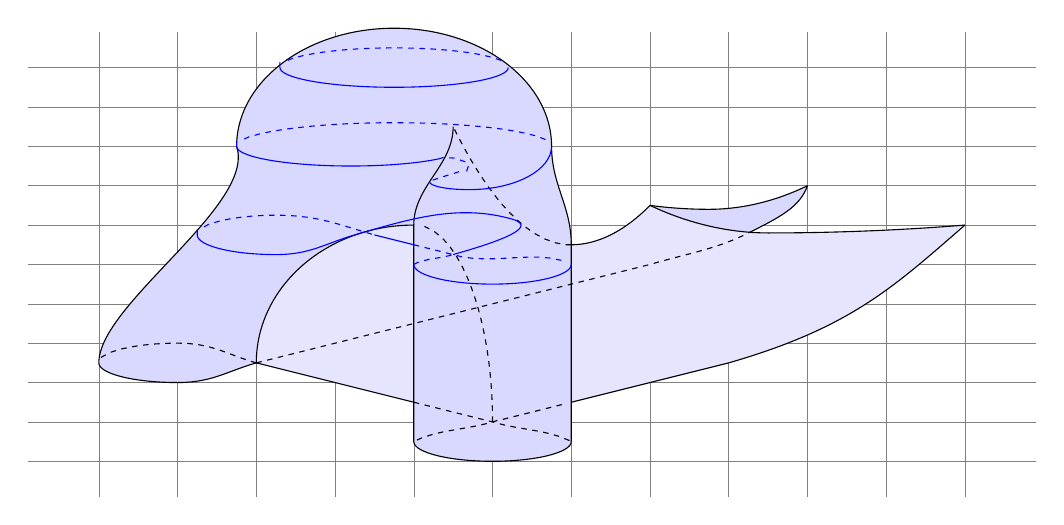
\begin{tikzpicture}[
			yscale = 0.5,
			% This decoration will be used to make portions of curves into "bouckground curves". It allows us to dash a portion of the curve.
			decoration={border, 
				segment length = 4pt, 	% determines the distance between consecutive ticks.
				amplitude = 2pt, 		% determines the length of the ticks.
				angle = 0  				% determines the angle between the ticks and the line of the path. 
				}, 
			% Styles
			contour line/.style={thin, blue}
				]
				
			% Colors
			\colorlet{surfacecolor1}{blue!15}
			\colorlet{surfacecolor2}{blue!10}	
			
			% The graphic
			\draw [step = 1cm, help lines] (-0.9,-0.9) grid (11.9, 10.9);
			
			% First we fill the surfaces with the background colors.
			% region 1
			\fill [color = surfacecolor1] (0, 2.5) .. controls (0, 4) and (2,6.5) .. (1.75,8)
				arc (180:0:2cm and 3cm)
				%.. controls (3, 9) and (3,10) .. (4,10)
				%.. controls (4.5,10) and (6,9.5) .. (6,8)
				to [out = 270, in = 90] (6, 5.5)
				-- (6,0.5)
				arc (360: 180: 1cm and 0.5cm)
				-- (4, 6)
				arc (90:180:2cm and 3.5cm)
				%.. controls (1, 2) and (1.5, 2) .. (1, 2)
				to [out = 210, in = 0] (1,2)
				arc (270: 180: 1cm and 0.5cm);
			
			% region 2
			\fill [color = surfacecolor1] (7, 6.5) parabola bend (8.5, 5.8) (8.25, 5.8) 
				to [out = 45, in = 260] (9, 7)
				parabola bend (7.75, 6.4) (7, 6.5);
			
			% region 3
			\fill [color = surfacecolor2] (4, 6) arc (90:180:2cm and 3.5cm)
				-- (4, 1.5) -- (4,6);
			
			% region 4
			\fill [color = surfacecolor2] (6, 5.5) parabola (7, 6.5) parabola bend (8.5, 5.8) (11, 6)
				to [out = 240, in = 30] (8, 2.5) -- (6, 1.5) -- (6, 5.5);
			
			
			% Now we draw the lines of the surface
			%first around region 1
			\draw (0, 2.5) .. controls (0, 4) and (2,6.5) .. (1.75,8)
				arc (180:0:2cm and 3cm)
				%.. controls (3, 9) and (3,10) .. (4,10)
				%.. controls (4.5,10) and (6,9.5) .. (6,8)
				to [out = 270, in = 90] (6, 5.5)
				-- (6,0.5)
				arc (360: 180: 1cm and 0.5cm)
				-- (4, 6)
				arc (90:180:2cm and 3.5cm)
				%.. controls (1, 2) and (1.5, 2) .. (1, 2)
				to [out = 210, in = 0] (1,2)
				arc (270: 180: 1cm and 0.5cm);
			
			% then the rest 
			\draw (2,2.5) -- (4,1.5) 
				decorate {-- (5,1) to [out = -30, in = 135] (6,0.5)
					  (4,0.5) to [out = 45, in = 210] (5,1) -- (6,1.5)} 
				-- (8, 2.5) to [out = 30, in = 240] (11, 6);
				% then off to cusp points
			\draw decorate { (5, 1) arc (0:90:1cm and 5cm)};
			\draw decorate {(2,2.5) -- (7,5) to [out = 30, in = 225] (8.25, 5.8)} to [out = 45, in = 260] (9, 7) ;
			\draw decorate {(2,2.5) to [out = 150, in = 0] (1,3) arc (90:180:1cm and 0.5cm)};
			% cusp
			\draw (4, 6) to [out = 90, in = 270] (4.5, 8.5);
			\draw (6, 5.5) decorate { parabola (4.5, 8.5)} (6, 5.5) parabola (7, 6.5)
				parabola bend (7.75, 6.4) (9, 7);
			\draw (7, 6.5) parabola bend (8.5, 5.8) (11, 6);
			
			% now the contour lines
			% the first contour line
			\draw [contour line] (2.3, 10) arc (180:360:1.45cm and 0.5cm)
				decorate {(2.3, 10) arc (180:0:1.45cm and 0.5cm)};
			
			
			% the second contour line
			\draw [contour line] (1.75,8) arc (180:320:1.45cm and 0.5cm)
				decorate {to [out = 30,in = 135](4.65, 7.6) to [out = -45, in = 45] (4.2, 7.1) }
				arc (180:270:0.5cm and 0.2cm) to [out = 0, in = -90] (5.75,8)
			;
			\draw [contour line] decorate {(1.75,8) arc (180:0:2cm and 0.6cm)};
			
			% the third contour line
			\draw [contour line] 
				decorate {(1.25, 5.75) arc (180:90: 1cm and 0.5cm) to [out = 0, in = 150] (3.5,5.75)}
				 -- (4, 5.5) 
				decorate {-- (4.5,5.25) to [out = -30, in = 135] (6,5)}
				arc (360: 180: 1cm and 0.5cm)
				decorate { to [out = 45, in = 210] (4.5,5.25)};
			
			\draw [contour line] 
			 (1.25, 5.75) arc (180: 270: 1cm and 0.5cm) to [out = 0, in = 210] (3.25,5.75)
			 	 to [out = 30, in = 150] (5.25, 6.15) to [out = -30,in = 30] (4.5, 5.25);
			
			%\draw (0,3) decorate {to (2,3)} -- (3,4);
				
		\end{tikzpicture}
		\end{center}	
	\caption{squashed, with all contour lines}
	%\label{fig:label}
\end{figure}


\tikzexternaldisable

The 1-morphism $ev^L$ of $\FrBord_2$ itself has a left adjoint $ev^{LL}$, and similarly $ev^R$ has a right adjoint, and so on.  The 1-morphism $coev$ also has a chain of left and right adjoints.  We therefore have two infinite series of adjunctions, as follows:

\begin{figure}[htbp]
	\begin{center}
		\begin{tikzpicture}[
			% This decoration will be used to make portions of curves into "bouckground curves". It allows us to dash a portion of the curve.
			%xscale = 0.75,
			decoration={border, 
				segment length = 4pt, 	% determines the distance between consecutive ticks.
				amplitude = 2pt, 		% determines the length of the ticks.
				angle = 0  				% determines the angle between the ticks and the line of the path. 
				}, 
			% Styles
			contour line/.style={thin, blue}
				]
				
			% Colors
			\colorlet{surfacecolor1}{black!12}
			\colorlet{surfacecolor2}{black!5}	
			
			% The graphic
			\draw [step = 1cm, help lines] (-0.9,-0.9) grid (11.9, 10.9);
			
			\begin{scope}[scale=0.75]			
				% adding fuzz
				\draw [fuzzright] (0,2.5) arc (180:270: 1cm and 0.5cm) to [out = 0, in = 210] (2,2.5)
					-- (4.5, 1.25);
				\draw [fuzzleft] (0,2.5) arc (180:90: 1cm and 0.5cm);
				\draw [fuzzright] (4, 0.5) arc (180:360: 1cm and 0.5cm);
				\draw [fuzzleft] (4, 0.5) arc (180:90: 1cm and 0.5cm);
				
				\draw [fuzzright] (6, 1.5) -- (8, 2.5) to [out = 30, in = 240] (11, 6);
				\draw [fuzzright]	 (8.25, 5.8) to [out = 45, in = 260] (9, 7);
			
			% First we fill the surfaces with the background colors.
			% region 1
			\fill [color = surfacecolor1] (0, 2.5) .. controls (0, 4) and (2,6.5) .. (1.75,8)
				arc (180:0:2cm and 3cm)
				%.. controls (3, 9) and (3,10) .. (4,10)
				%.. controls (4.5,10) and (6,9.5) .. (6,8)
				to [out = 270, in = 90] (6, 5.5)
				-- (6,0.5)
				arc (360: 180: 1cm and 0.5cm)
				-- (4, 6)
				arc (90:180:2cm and 3.5cm)
				%.. controls (1, 2) and (1.5, 2) .. (1, 2)
				to [out = 210, in = 0] (1,2)
				arc (270: 180: 1cm and 0.5cm);
			
			% region 2
			\fill [color = surfacecolor1] (7, 6.5) parabola bend (8.5, 5.8) (8.25, 5.8) 
				to [out = 45, in = 260] (9, 7)
				parabola bend (7.75, 6.4) (7, 6.5);
			
			% region 3
			\fill [color = surfacecolor2] (4, 6) arc (90:180:2cm and 3.5cm)
				-- (4, 1.5) -- (4,6);
			
			% region 4
			\fill [color = surfacecolor2] (6, 5.5) parabola (7, 6.5) parabola bend (8.5, 5.8) (11, 6)
				to [out = 240, in = 30] (8, 2.5) -- (6, 1.5) -- (6, 5.5);
			
			
			% Now we draw the lines of the surface
			%first around region 1
			\draw (0, 2.5) .. controls (0, 4) and (2,6.5) .. (1.75,8)
				arc (180:0:2cm and 3cm)
				%.. controls (3, 9) and (3,10) .. (4,10)
				%.. controls (4.5,10) and (6,9.5) .. (6,8)
				to [out = 270, in = 90] (6, 5.5)
				-- (6,0.5)
				arc (360: 180: 1cm and 0.5cm)
				-- (4, 6)
				arc (90:180:2cm and 3.5cm)
				%.. controls (1, 2) and (1.5, 2) .. (1, 2)
				to [out = 210, in = 0] (1,2)
				arc (270: 180: 1cm and 0.5cm);
			
			% then the rest 
			\draw (2,2.5) -- (4,1.5) 
				decorate {-- (5,1) to [out = -30, in = 135] (6,0.5)
					  (4,0.5) to [out = 45, in = 210] (5,1) -- (6,1.5)} 
				-- (8, 2.5) to [out = 30, in = 240] (11, 6);
				% then off to cusp points
			\draw decorate { (5, 1) arc (0:90:1cm and 5cm)};
			\draw decorate {(2,2.5) -- (7,5) to [out = 30, in = 225] (8.25, 5.8)} to [out = 45, in = 260] (9, 7) ;
			\draw decorate {(2,2.5) to [out = 150, in = 0] (1,3) arc (90:180:1cm and 0.5cm)};
			% cusp
			\draw (4, 6) to [out = 90, in = 270] (4.5, 8.5);
			\draw (6, 5.5) decorate { parabola (4.5, 8.5)} (6, 5.5) parabola (7, 6.5)
				parabola bend (7.75, 6.4) (9, 7);
			\draw (7, 6.5) parabola bend (8.5, 5.8) (11, 6);
			
			% now the contour lines
			% the first contour line
			\draw [contour line] (2.3, 10) arc (180:360:1.45cm and 0.5cm)
				decorate {(2.3, 10) arc (180:0:1.45cm and 0.5cm)};
			
			
			% the second contour line
			\draw [contour line] (1.75,8) arc (180:320:1.45cm and 0.5cm)
				decorate {to [out = 30,in = 135](4.65, 7.6) to [out = -45, in = 45] (4.2, 7.1) }
				arc (180:270:0.5cm and 0.2cm) to [out = 0, in = -90] (5.75,8)
			;
			\draw [contour line] decorate {(1.75,8) arc (180:0:2cm and 0.6cm)};
			
			% the third contour line
			\draw [contour line] 
				decorate {(1.25, 5.75) arc (180:90: 1cm and 0.5cm) to [out = 0, in = 150] (3.5,5.75)}
				 -- (4, 5.5) 
				decorate {-- (4.5,5.25) to [out = -30, in = 135] (6,5)}
				arc (360: 180: 1cm and 0.5cm)
				decorate { to [out = 45, in = 210] (4.5,5.25)};
			
			\draw [contour line] 
			 (1.25, 5.75) arc (180: 270: 1cm and 0.5cm) to [out = 0, in = 210] (3.25,5.75)
			 	 to [out = 30, in = 150] (5.25, 6.15) to [out = -30,in = 30] (4.5, 5.25);
			
			
%			\begin{scope}[xshift = -4cm, yshift =2.5cm, scale = 0.75]
%				% now the contour lines
%				% the first contour line
%				\draw [contour line] (2.3, 10) arc (180:360:1.45cm and 0.5cm)
%					 {(2.3, 10) arc (180:0:1.45cm and 0.5cm)};
%			
%			
%				% the second contour line
%				\draw [contour line] (1.75,8) arc (180:320:1.45cm and 0.5cm)
%					 {to [out = 30,in = 135](4.65, 7.6) to [out = -45, in = 45] (4.2, 7.1) }
%					arc (180:270:0.5cm and 0.2cm) to [out = 0, in = -90] (5.75,8)
%				;
%				\draw [contour line]  {(1.75,8) arc (180:0:2cm and 0.6cm)};
%			
%				% the third contour line
%				\draw [contour line] 
%					 {(1.25, 5.75) arc (180:90: 1cm and 0.5cm) to [out = 0, in = 150] (3.5,5.75)}
%					 -- (4, 5.5) 
%					 {-- (4.5,5.25) to [out = -30, in = 135] (6,5)}
%					arc (360: 180: 1cm and 0.5cm)
%					 { to [out = 45, in = 210] (4.5,5.25)};
%			
%				\draw [contour line] 
%				 (1.25, 5.75) arc (180: 270: 1cm and 0.5cm) to [out = 0, in = 210] (3.25,5.75)
%				 	 to [out = 30, in = 150] (5.25, 6.15) to [out = -30,in = 30] (4.5, 5.25);
%			\end{scope}
		\end{scope}
			
			% now for some braces
		%	\draw [thick, decoration={brace, amplitude=3pt}]  decorate {(6.5, 10.5) -- (6.5,6.5)};
		%	\node at (7.5,8.5) {\small some math};
		%	\draw [thick, decoration={brace, amplitude=3pt}]  decorate {(11.5, 6.5) -- (11.5,1.5)};	
		%	\node at (12, 4) {\small more};			
			
		
		% Now the 2D diagrams
		\begin{scope}[xshift = 7cm, yshift = 2cm]
			
						% ev^L
						\draw[linestyle,fuzzright] (4,7) to [looseness=1.6,out = 180, in = 180] (4,6);
						\begin{pgfonlayer}{background}
							\draw[->,outstyle] (4,7) -- +(0:\arrowlength);
							\draw[->,outstyle] (4,6) -- +(0:\arrowlength);
						\end{pgfonlayer}
						
						% the first morphism	
						\draw [thick, ->] (3, 5.75) -- (3, 4.75);
							\draw[linestyle, fill=\fillcolor, yshift = 0.5*\smcirclerad] (3.5,5.25) 
								to [looseness=1.6, out=180, in=190] +(90:0.75*\smcirclerad)
								to [looseness=1.6, out=10, in=-10] +(90:-2.5*\smcirclerad)
								to [looseness=1.6, out=170, in=180] +(90:.75*\smcirclerad)
								to [looseness=1.55, out=0, in=0] +(90:\smcirclerad);
						\node at (4,5.5) {\small $R$};

						% ev^R ev + ev^L
						\draw[linestyle,fuzzright] (4,4.5) to [looseness=1.6,out = 180, in = 180] (4,3.5);
							\begin{pgfonlayer}{background}
								\draw[->,outstyle] (4,4.5) -- +(0:\arrowlength);
								\draw[->,outstyle] (4,3.5) -- +(0:\arrowlength);
							\end{pgfonlayer}
						\draw[yshift = \smcirclerad, linestyle, fuzzright] (2,4) 
							to [looseness=1.6, out=180, in=190] +(90:1.5*\smcirclerad)
							to [looseness=1.6, out=10, in=-10] +(90:-5*\smcirclerad)
							to [looseness=1.6, out=170, in=180] +(90:1.5*\smcirclerad)
							to [looseness=1.55, out=0, in=0] +(90:2*\smcirclerad);

						% the second morphism	
						\draw [thick, ->] (3, 3.25) -- (3, 2.25);
						\node at (3.5,2.75) {\small Isom};
							
						% ev^R ev + ev^L (deformed)
						\draw[linestyle,fuzzright] (4,2) to [looseness=1.6,out = 180, in = 180] (4,1);
								\begin{pgfonlayer}{background}
									\draw[->,outstyle] (4,2) -- +(0:\arrowlength);
									\draw[->,outstyle] (4,1) -- +(0:\arrowlength);
								\end{pgfonlayer}
						\draw[linestyle,fuzzright] (2.5, 2) -- (1.75,2)
								to [looseness=2,out = 180, in = 90] (2, 2.25)
									-- (2, 0.75)
									to [looseness=2,out = 270, in = 180] (1.75,1)
									-- (2.5, 1) arc (-90:90:0.5cm);
						
						% the third morphism			
						\draw [thick, ->] (3, 0.75) -- (3, -0.25);
						\begin{scope}[xshift = 3.5cm, yshift = 0.0cm, scale = 0.65]
							\filldraw[linestyle,fill=\fillcolor] 
							(0,0) .. controls (.25,.25) and (.75,.25) .. (1,0)
								.. controls (.75,.25) and (.75,.75) .. (1,1)
								.. controls (.75,.75) and (.25,.75) .. (0,1)
								.. controls (.25,.75) and (.25,.25) .. (0,0);
						\draw[linestyle,fuzzright]
							(0,0) .. controls (.25,.25) and (.75,.25) .. (1,0);
						\draw[linestyle,fuzzleft]
							(0,1) .. controls (.25,.75) and (.75,.75) .. (1,1);
						\begin{pgfonlayer}{background}
							\draw[->,outstyle] (1,1) -- +(45:\arrowlength);
							\draw[->,outstyle] (1,0) -- +(-45:\arrowlength);
						\end{pgfonlayer}
						\end{scope}
						

						% ev^R
							\draw[linestyle,fuzzright] (4, -0.5) -- (1.75, -0.5)
								to [looseness=2,out = 180, in = 90] (2, -0.25)
								-- (2, -1.75)
								to [looseness=2,out = 270, in = 180] (1.75,-1.5)
								-- (4, -1.5);
							\begin{pgfonlayer}{background}
								\draw[->,outstyle] (4,-0.5) -- +(0:\arrowlength);
								\draw[->,outstyle] (4,-1.5) -- +(0:\arrowlength);
							\end{pgfonlayer}

		\end{scope}	
			
				
						
							
		\end{tikzpicture}
		\end{center}	
	\caption{.... }
	%\label{fig:label}
\end{figure}



\begin{figure}[htpb]
	\begin{center} 
		\begin{tikzpicture}[
	%		fuzzright/.style={line width=\fuzzwidth,\fuzzcolor}
	%        preaction={draw,line width=\fuzzwidth,\fuzzcolor,decoration={curveto, amplitude=0,raise=-.3*\fuzzwidth}}}%,
	        %fuzzleft/.style={preaction={draw,line width=\fuzzwidth,\fuzzcolor,decorate,decoration={curveto,amplitude=0,raise=.5*\fuzzwidth}}}
			]
		
	
			% ev^L
			\draw[linestyle,fuzzright] (4,7) to [looseness=1.6,out = 180, in = 180] (4,6);
			\begin{pgfonlayer}{background}
				\draw[->,outstyle] (4,7) -- +(0:\arrowlength);
				\draw[->,outstyle] (4,6) -- +(0:\arrowlength);
			\end{pgfonlayer}
	
%			\draw[linestyle, fill=\fillcolor] (2,4) 
%				to [looseness=1.6, out=180, in=190] +(90:1.5*\smcirclerad)
%				to [looseness=1.6, out=10, in=-10] +(90:-5*\smcirclerad)
%				to [looseness=1.6, out=170, in=180] +(90:1.5*\smcirclerad)
%				to [looseness=1.55, out=0, in=0] +(90:2*\smcirclerad);
			
			% ev^R ev + ev^L
			\draw[linestyle,fuzzright] (4,4.5) to [looseness=1.6,out = 180, in = 180] (4,3.5);
				\begin{pgfonlayer}{background}
					\draw[->,outstyle] (4,4.5) -- +(0:\arrowlength);
					\draw[->,outstyle] (4,3.5) -- +(0:\arrowlength);
				\end{pgfonlayer}
			\draw[yshift = \smcirclerad, linestyle, fuzzright] (2,4) 
				to [looseness=1.6, out=180, in=190] +(90:1.5*\smcirclerad)
				to [looseness=1.6, out=10, in=-10] +(90:-5*\smcirclerad)
				to [looseness=1.6, out=170, in=180] +(90:1.5*\smcirclerad)
				to [looseness=1.55, out=0, in=0] +(90:2*\smcirclerad);
	
			
			% ev^R ev + ev^L (deformed)
			\draw[linestyle,fuzzright] (4,2) to [looseness=1.6,out = 180, in = 180] (4,1);
					\begin{pgfonlayer}{background}
						\draw[->,outstyle] (4,2) -- +(0:\arrowlength);
						\draw[->,outstyle] (4,1) -- +(0:\arrowlength);
					\end{pgfonlayer}
			\draw[linestyle,fuzzright] (2.5, 2) -- (1.75,2)
					to [looseness=2,out = 180, in = 90] (2, 2.25)
						-- (2, 0.75)
						to [looseness=2,out = 270, in = 180] (1.75,1)
						-- (2.5, 1) arc (-90:90:0.5cm);
			
			
	
			% ev^R
				\draw[linestyle,fuzzright] (4, -0.5) -- (1.75, -0.5)
					to [looseness=1.7,out = 180, in = 90] (2, -0.25)
					-- (2, -1.75)
					to [looseness=1.7,out = 270, in = 180] (1.75,-1.5)
					-- (4, -1.5);
				\begin{pgfonlayer}{background}
					\draw[->,outstyle] (4,-0.5) -- +(0:\arrowlength);
					\draw[->,outstyle] (4,-1.5) -- +(0:\arrowlength);
				\end{pgfonlayer}
		
			
		
		\end{tikzpicture}
	\end{center}
	\caption{.... }
\end{figure}


\end{document}
	
	